\section{Introduction}
\protect\label{section:intro}

\engdate

This report describes steps taken to analyse observational data from the
{\rem} (Rapid Eye Mount) telescope and camera equipment in La Silla, Chile, as
operated by the Red Dots Project. This work commenced in March 2015.
\citep{reddotsspace20}. However the data collection for the project did not
start until mid-July 2017.

The {\rem} telescope has been set up to take a series of automatic
observations of patches of sky on a nearly nightly basis. The main concern of
the Red Dots Project is of {\rdwarf} stars and as the {\rem} observatory is
concurrently used for other projects, for example \citet{giannini18}, this
report focuses on the {\rdwarf} targets designated by the Red Dots Project.

The first observations of {\rdwarf} stars took place in mid-2017. All
observations ceased on March 2020 due to the Coronavirus pandemic but were
restarted in October 2020 and continued up until April 2022.

The original objectives of the work documented in this report are:
\begin{enumerate}
  \item To set up a pipeline for automatic analysis and processing of the data.
  \item To evaluate to what degree reliable photometry, together with an
  estimate of the error bars, can be obtained in relation to the targets of
  interest.
  \item If accuracy and reliability of the photometry permit, obtain periodic
  data for the target stars of particular interest.
\end{enumerate}

Other supplementary objectives came to light over the course of the work. An
early example of this was obtaining a rotation period for \ross. As noted in
Section \ref{section:introross}, there is a little lack of clarity and some
contradictions in the published rotation period, so some work was undertaken to
establish the rotation period of {\ross} from existing data sources and then
attempt to recover the same period from  no rotation period is currently
reported for \ross, so an early benchmark was identified by attempting to
recover this period from various sources listed in the papers discussing {\ross}
and comparing the result with that obtained from various iterations of the data
analysis undertaken with the {\rem} data.

\subsection{The {\rem} telescope}
\protect\label{section:remscope}

The {\rem} observatory at La Silla was initially set up in 2003
\citep{antonelli05} consisting of the the REMIR near-infrared camera and the
visible light camera, ROSS. Light from the 60cm telescope is split at 1 $\mu$m into two beams
by a dichroic element. The light with wavelength greater than this passes to the
REMIR near-infrared camera and the smaller wavelengths to the ROSS camera.

\subsubsection{The REMIR camera}

The commissioning of the REMIR telescope is described in \citet{conconi04} and
\citet{vitali03}. There was some restyling of the cryogenics to overcome some
problems which are described in \citet{vitali06}.

Light to the REMIR telescope is split between 3 filters, \texttt{H}, \texttt{J}
and \texttt{K} with one of seven of dither patterns. Images are returned as
512x512 arrays with reduction already carried out using PREPROCESS software
\citep{dipaola01}, as described in \citet{calzoletti05}.

This has generally performed satisfactorily, being used in a number of studies,
for example \citet{dammando11} and  \citet{davanzo06}, which latter also used the ROSS camera.

The REMIR observations were discontinued at the beginning of June 2019 due to a
system fault. They were restarted at the beginning of February 2021.

\subsubsection{The ROSS and ROSS2 cameras}

The performance of the ROSS camera was not satisfactory and in 2015 it
was replaced by the ROSS2 camera system, described in outline at
\citet{reminaf7} and in more detail in \citet{molinari14}.

The visible light portion of the light from the telescope is split between 4
Sloan-style filters and projected onto quadrants of a 2048x2048 CCD array, which
is an ANDOR Ikon-L series chip. The names, quadrants and bandwidths of the 4
filters are set out in Table \ref{table:ros2quad}.

\begin{table}[!htbp]
\begin{center}
\begin{tabular}{llrr} \hline
Filter & Quadrant & Low bw (nm) & High bw (nm) \\\hline
\texttt{g'} & Upper Right & 400 & 550 \\
\texttt{r'} & Lower Right & 550 & 700 \\
\texttt{i'} & Upper Left & 700 & 820 \\
\texttt{z'} & Lower Left & 820 & 1000 \\
\hline
\end{tabular}
\end{center}
\caption{The four ROSS2 filters, quadrant used on the CCD chip, low and high
bandwidth in nm. Hereinafter the filters are referred to as \texttt{g},
\texttt{r}, \texttt{i} and \texttt{z} respectively and the quadrants as UR, LR,
UL and LL.} \protect\label{table:ros2quad}
\end{table}

The images from the visible light telescope are nominally 1024 by 1924 pixels,
although the effective area is only in the region of 900 by 900
pixels varying for each filter as the settings are periodically adjusted.
As a consequence of the construction of the ROSS2 camera, all of the visible
light images are taken at exactly the same time with exactly the same
exposure, viewing exactly the same patch of sky. In Fig. \ref{fig:showusedccd}
is shown the areas on the CCD used by various filters at various times.

\begin{figure}[!htbp]
\begin{center}
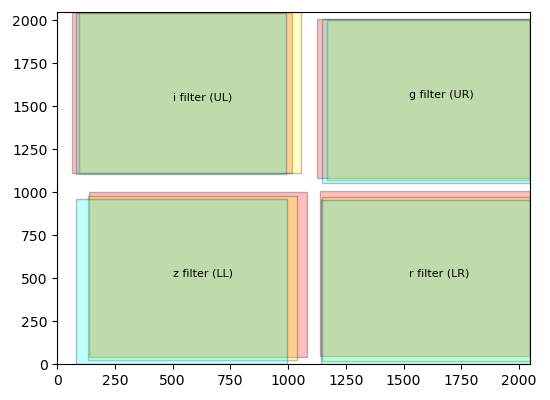
\includegraphics[scale=1]{images/showusedccd.png} \\
\end{center}   
\caption{This figure sets out the areas of the CCD used by the ROSS2
telescope which are used for the various filters at various times after
adjustment of the telescope. The area shaded in red is that prior to July 2015, the yellow shaded area is between
then and March 2019 and the blue part after then. The bulk of the area is
common to all of the configurations as can be seen. Note that all of the
{\rdwarf} observations, with which this report is concerned, start in 2017, well
after the first reconfiguration.} \protect\label{fig:showusedccd}
\end{figure}

Bias frames are taken daily for the visible light filters, usually 5 at
approximately 11:30 am and flat field frames nearly as often, usually 3 at a
time as the sky fades. A monthly master flat and bias file for each visible
light filter is also constructed from the daily flat and bias frames.

As noted above, the ROSS2 observations were discontinued from 23 March 2020 due
to the Coronavirus pandemic and were restarted on 22 October 2020.

The ROSS2 camera results have been used in a number of other projects from the
Red Dots project for example in \citet{frasca20} and \citet{riverasandoval18}
but for a limited set of dates only. The data available for the Red Dots project
is very much more extensive than the other papers, covering nearly 3 years from mid-2017 to March 2020 and then
further observations being added every day from the end of October 2020
continuing through to April 2022.

\subsection{Targets}

The primary targets for the Red Dots project are \rdwarf s, although
observations are made of other types of star during the course of each night
for other projects. In this report, only the {\rdwarf} observations are
considered. As the REMIR observations have already been processed, much of this report
focuses upon reduction of the ROSS2 visible light telescope.

The three main targets of the Red Dots REM observations are \prox, {\bstar} and
\ross, all \rdwarf s of spectral types M6, M4 and M3.5 respectively and at
nearest, fourth nearest and eleventh nearest known stellar objects to the solar
system. In Fig. \ref{fig:rdwarfhist} is shown the distribution of observations
of these targets.

\begin{figure}[!htbp]
\begin{center}
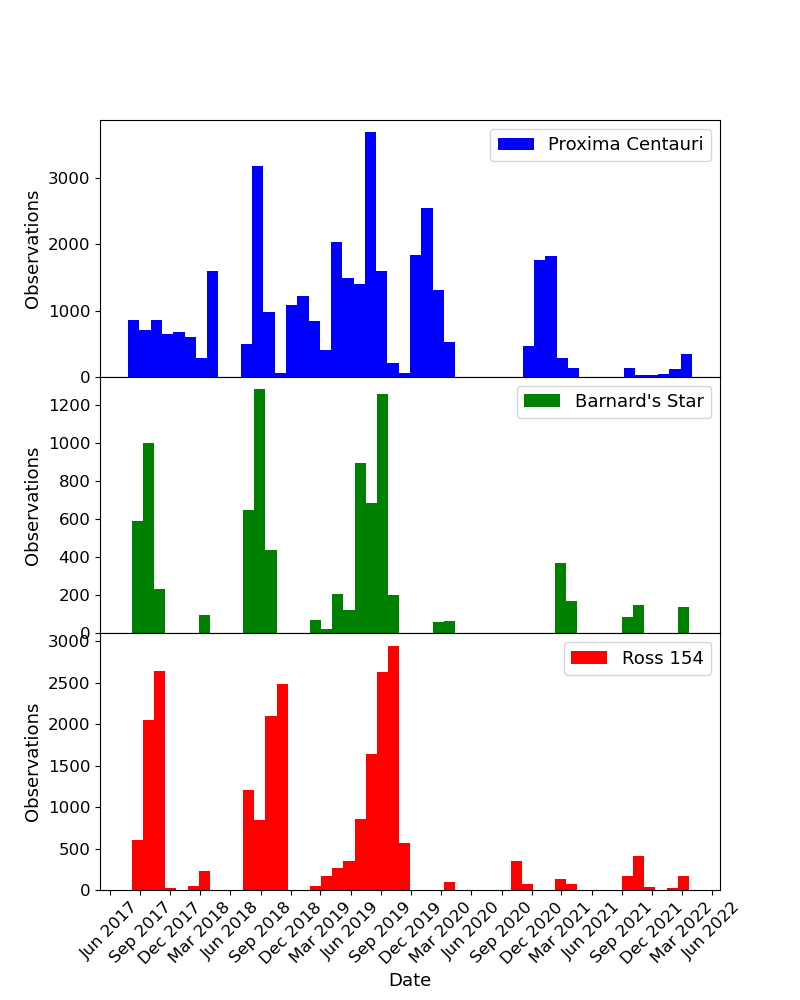
\includegraphics[scale=0.60]{images/rdwarfhist.png} \\
\end{center}   
\caption{This figure shows the distribution of observations of the three
{\rdwarf} targets to date, with {\prox} observations in the top pane, {\bstar}
in the middle pane and {\ross} in the bottom pane.}
\protect\label{fig:rdwarfhist}
\end{figure}

\subsubsection{\prox}

{\prox} is of perennial interest as the closest star to the solar system, at 1.30197 pc. It is of spectral type M5.5.
Calculations of the the rotation period of {\prox} have varied over the years,
most recently in \citet{collins17} in which the rotation period was calculated
at 82.6 $\pm$ 0.1 days, based primarily on photometric evidence, with some
support from spectroscopic analysis of an {\ha} peak.

There has been much study of planets detected, in particular in 2016 a planet of 1.3 Earth mass was reported
in the habitable zone of \prox, known as {\prox} b. \citep{angladaescude16}.
Its orbital period was calculated as just over 11 days.

The frequent flare activity is unusual in a star of slow rotation like \prox,
previous studies such as In \citet{mohanty03} setting out the correlation
between the projected rotational velocity {\vsini} and the
activity in mid-M to L-dwarfs, In \citet{vida19} the flaring activity was
calculated as 1.49 events per day. with ``superflares'' approximately 3 times a
year and flares a magnitude larger every other year.

As shown in Fig. \ref{fig:rdwarfhist}, the bulk of
the observations taken by the Red Dots project are of \prox.

\subsubsection{\bstar}
\protect\label{section:introbstar}
{\bstar} is, at 1.8282 pc, the fourth closest star to the solar system after {\prox} and Alpha Centauri A and B.
It is of spectral type M4. It is particularly notable for its very large proper motion of {-}802.803 mas/yr
in Right Ascension and 10,362.542 mas/yr in Declination, the largest of all stars relative to the solar system.
This is combined with a high radial velocity of {-}110.6 km/s \citep{bobylev17}.
The high radial velocity of {\bstar} will bring it close enough to the solar
system to rival or perhaps surpass {\prox} in approximately 10,000 years as estimated by \citet{bobylev10}.

Its rotation period has been progressively given as 130 days in \citet{benedict98}, 148.6 days in \citet{suarezmascareno15} 
and 145 $\pm$ 15 days in \citet{toledopadron18}. Activity is low, as noted in the latter.

Due to the high proper motion, care has to be taken to correctly take this into account when identifying it in images.

\subsubsection{\ross}
\protect\label{section:introross}
{\ross} is 2.976 pc distant, of spectral type M3.5. It has a reasonably high
proper motion of $-637.02$ mas/yr in Right Ascension and  {–}191.64 mas/yr
in Declination and a radial velocity of {–}10.7 km/s \citep{vanleeuwen07}.
The strong activity is noted in \citet{wargelin08}.

As discussed in the draft paper included herewith, there is a wide variation in
some of the parameters for {\ross}, in particular the value of \vsini, the
radius and the rotation period. It became clear that an early benchmark of the work on the
{\rem} data would be clarification of the rotation period.

\subsection{Proper Motions and caveats}
\protect\label{section:propermotions}
As all the target objects are amongst the closest objects outside the solar
system, they all have particularly large proper motions. Care must be taken to
track the proper motions of the targets and any adjacent objects.

The resolution of the ROSS2 camera is such that successive pixels
are approximately 0.6 arc-seconds apart (about 4.9 for Declination values, 6.9
for Right Ascension values but that varies a little with declination). This
means that proper motions of less than 20 milliarcseconds / year may be safely
disregarded which eliminates all but a handful of objects\footnote{18 objects
altogether, 10 in the vicinity of \prox, 1 in the vicinity of {\bstar} and 7 in
the vicinity of \ross.} in the vicinity of the targets from a need to track proper
motions for the bulk of other objects.

In Fig. \ref{fig:proxpm}, Fig. \ref{fig:bspm} and Fig. \ref{fig:rosspm} are
illustrated the proper motions \prox, {\bstar} and {\ross} respectively against
the immediate backgrounds.

\begin{figure}[!htbp]
\begin{center}
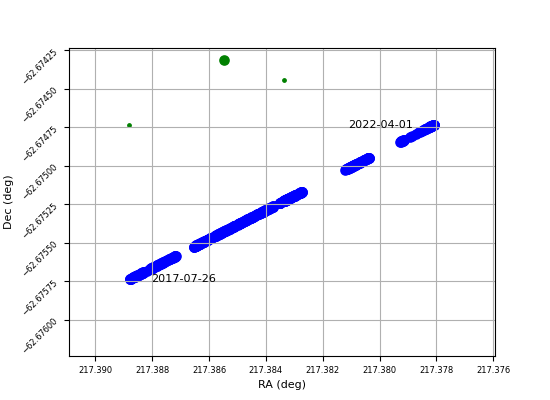
\includegraphics[scale=0.9]{images/pmprox.png} \\
\end{center}   
\caption{This figure tracks the proper motion of {\prox} against the immediate
background stars, showing start and end dates of the observations at the time
of writing, the gaps showing the periods where observations were not taken..} \protect\label{fig:proxpm}
\end{figure}

\begin{figure}[!htbp]
\begin{center}
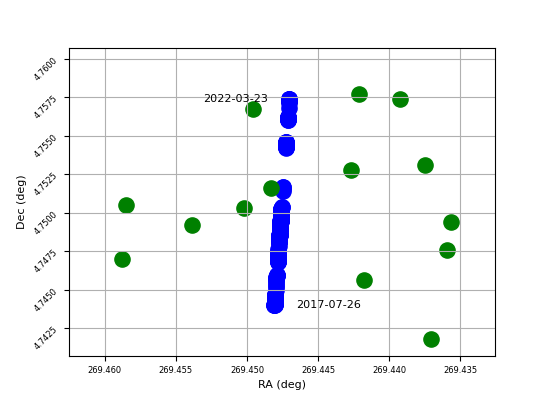
\includegraphics[scale=1]{images/pmbstar.png} \\
\end{center}   
\caption{This figure tracks the proper motion of {\bstar} against the immediate
background stars, showing start and end dates of the observations at the time
of writing, the gaps showing the periods where observations were not taken. The proper motion of {\bstar} is
extremely large and the scale is not the same as in Fig. \ref{fig:proxpm} or
Fig.  \ref{fig:rosspm} in consequence. Proper motion on Declination is so large
that the scale is reduced by a factor of 10 from that in Right Ascension.} \protect\label{fig:bspm}
\end{figure}

\begin{figure}[!htbp]
\begin{center}
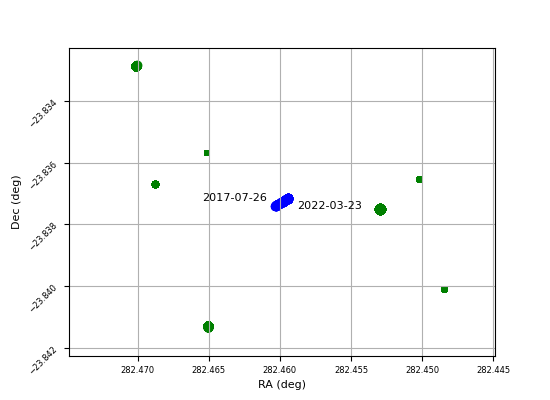
\includegraphics[scale=0.9]{images/pmross.png} \\
\end{center}   
\caption{This figure tracks the proper motion of {\ross} against the immediate
background stars, showing start and end dates of the observations at the time
of writing, the gaps showing the periods where observations were not taken.
The scale is the same as in Fig. \ref{fig:proxpm} (but not the same as in Fig. \ref{fig:bspm}).}
\protect\label{fig:rosspm}
\end{figure}

\clearpage
